%TEX root = ./overwiew.tex

\documentclass[varwidth]{standalone}
% http://texample.net/tikz/examples/inertial-navigation-system/
\usepackage{amsmath}
\usepackage[makeroom]{cancel}
\usepackage{tikz}
\usetikzlibrary{positioning}
\usetikzlibrary{decorations.pathreplacing}
\usetikzlibrary{shapes,arrows}

\begin{document}

\tikzstyle{module}=[draw, fill=blue!20, text width=5em, text centered, minimum height=2cm]
\tikzstyle{module_def}=[fill=yellow!20,rounded corners, draw=black!50, dashed]
\tikzstyle{signal_name} = [above, text width=10em]
\tikzstyle{module_name} = [above right, text width=10em]

\def\blockdist{3.5cm}
\def\edgedist{1.5cm}

\pgfdeclarelayer{background}
\pgfdeclarelayer{foreground}
\pgfsetlayers{background,main,foreground}

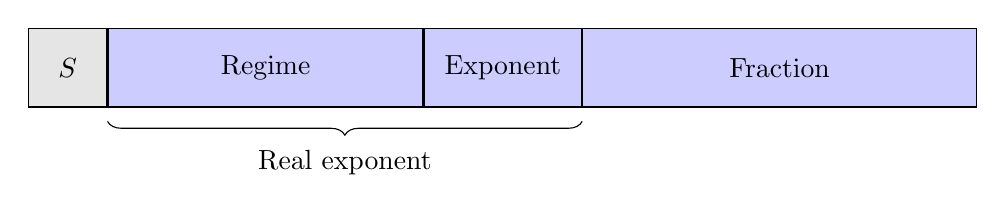
\begin{tikzpicture}
    \node [draw, fill=blue!20, minimum width=4cm, minimum height=1cm] (regime) {Regime};
    \node [draw, fill=blue!20, minimum width=2cm, minimum height=1cm] (exponent) [right=0cm of regime] {Exponent};
    \node [draw, fill=blue!20, minimum width=5cm, minimum height=1cm] (fraction) [right=0cm of exponent] {Fraction};
    \node [draw, fill=gray!20, minimum width=1cm, minimum height=1cm] (sign) [left=0cm of regime] {$S$};

    \draw [decorate, decoration={brace, amplitude=5pt,mirror, raise=5pt}] (regime.south west) -- (exponent.south east) node[midway,yshift=-2em] {Real exponent};
\end{tikzpicture}

\end{document}

